
% PROCESS =========================================================================
\subsection{Processes}
    Each application, including all its components runs in a single process. The 
    application object from the framework is always in memory (singleton object); 
% PRIORITIES =======================================================================
\subsection{Priorities}
    Processes are organized in priority levels depending on the state of its components.
    When there is some lack of resources processes are automatically terminated. 

    \begin{figure}[h]
    \centering
    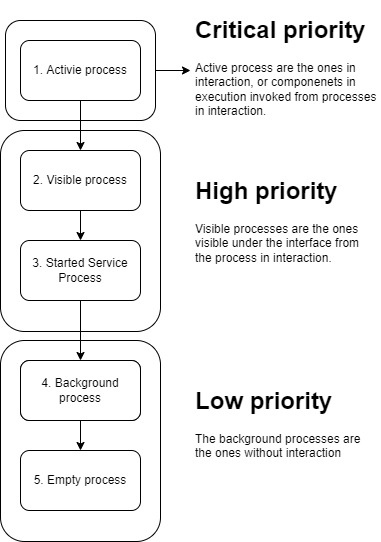
\includegraphics[width=0.4\linewidth]{figures/02_process_priority.png}
    \caption{Process priorities}
    \label{fig:process_priority}
    \end{figure}

% ACTIVITIES =======================================================================
\subsection{Activities}
    Usually show an user interface (using ViewGroups and Views) and inherit from android.app.Activity.
The activities execute a specific task in the application and the android always mantains a stack of 
activities. 

    Let's suppose that one activity inits another one. The first activity will go to the stack. When the 
back button is pressed, the first activity is retrieved from the stack. 

    An activity might be:
    \begin{itemize}
        \item active (runnning) - In interaction
        \item paused - Visible;
        \item Stopped - Non visible;
        \item Inactive (destroyed) - Without an instance object;
    \end{itemize}

    The android call lifecycle methods when there's a state transition.  



\subsubsection{In interaction vs Paused}
Let's suppose that we are running an active and then a dialog box pops up. Considering 
that the dialog box is managed by another activity, we can say that the previous activity is 
paused, but visible. The current activity (i.e the dialog box) is the active one. 

\subsubsection{Starting an activity}   
Before starting, take a look on the diagram below. This is the complete state diagram for android.

\begin{figure}[h]
    \centering
    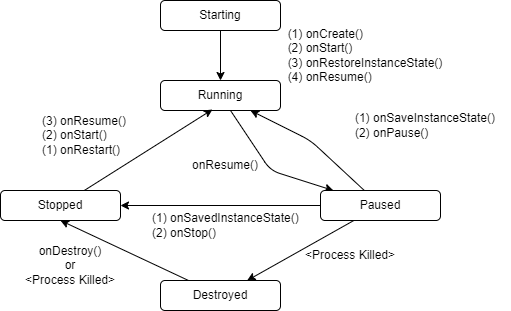
\includegraphics[width=0.8\linewidth]{figures/02_state_diagram.png}
    \caption{Activities State Diagram}
    \label{fig:state_diagram}
\end{figure}

Firstly the android system call life-cycle callbacks starting with the \textbf{onCreate()}. 

\begin{lstlisting}
// Always override
override fun onCreate(savedInstanceState: Bundle?){
    super.onCreate(savedInstanceState)
    val bt = findViewById<Button>(R.id.some_button)
    bt.setOnClickListener(this)
}
\end{lstlisting}

We should associate the listeners to interacion events in onCreate().


\subsubsection{Activity Navigation}
There are two criterias to the navigation:
\begin{itemize}
    \item Based on the past activated activity and the activity stack. This is usually 
    used when the user presses the \textbf{back button}.
    \item Based on a defined hierarchy. We can declare an activity parent in the manifest file 
    for each activity (except the one that starts the application); and a person can use the Up 
    button in the action bar to navigate.
\end{itemize}

% RESOURCES ========================================================================
\subsection{Resources}
The resources can be:
\begin{itemize}
    \item drawable - bitmaps, graphics, shapes, etc 
    \item anim - XML specifying animations between 2 configurations (tweens)
    \item color - colors (AARRGGBB) for many elements of the interface according to 
    state (pressed, focused, selected, ...)
    \item layout - screen organization 
    \item menu - options and context menus specifications 
    \item values - value collections with a name: string, arrays, colors, styles, dimensions,...
    \item xml - other XML files read with getXML()
\end{itemize}

\subsection{Events and listeners (IoC pattern)}

\subsubsection{Inversion of Control (IoC)}
IoC is the inversion control principle. Actually it's a principle, not a design pattern. 
This principle defines a basic characteristic of frameworks and it was popularized in 2004 by 
Robert C. Martin and Martin Fowler.  

Imagine that we have a code like this:

\begin{lstlisting}
public static void main(String[] args) {
    while (true) {
        BufferedReader userInputReader = new BufferedReader(
                new InputStreamReader(System.in));
        System.out.println("Please enter some text: ");
        try {
            System.out.println(userInputReader.readLine());
        } catch (IOException e) {
            e.printStackTrace();
        }
    }
}
\end{lstlisting}

The code is really simple: it will try to read the user input for undefined time and print in the console.
The main function/file has controls the program flow.  

Now consider that we've decided to use a GUI to do the same logic. The \textbf{framework is responsible for calling the user code.}
The framework is an extendable structure that provides the developer a set of specific points for injecting segments of the code.

\begin{tcolorbox}[title=IoC in short]
    In the case of frameworks that stick to the open/closed principle by 
    providing an extendable API, the role of the developer using the framework 
    boils down to defining their own set of custom classes, either by implementing 
    one or multiple interfaces provided by the framework or by inheriting from 
    existing base classes. In turn, instances of the classes are directly 
    instantiated from and called by the framework.
\end{tcolorbox}

\subsubsection{IoC in android}
In android the framework needs to listen the user code and execute it. Everytime a user makes an interaction, a message goes 
to a message queue, which is executed by a main thread (e.g UI thread). The main therad runs a 
loop that reads the message from the queue and makes a callback (life-cycle) or calls an event linstener (handler).

Here, the framework has the program flow. 


\subsection{Events generated by the interface}
Many views generate events, such as clicking in a button, changing focus, etc.  
We need to install listeners to these evets, by implementing the interfaces that describe them. 
Them implemented methods are called when the event occurs, such as:

\begin{itemize}
    \item onClick()
    \item onLongClick()
    \item onFocusChange()
    \item onKey()
    \item onTouch()
    \item onCreateContextMenu()
\end{itemize}

Defining a listerner is easy and can be defined in an activity: 

\begin{lstlisting}
// Listener defined in an activity
class ExampleActivity: Activity(), OnClickListener{
    ...
    val button = findViewById<Button>(R.id.corky);
    button.setOnClickListener(this);

}
// Implement the OnClickListener interface
override fun onClick(v: View){
    // Do something
}
\end{lstlisting}

As an anonymous object listener:
\begin{lstlisting}
override onCreate(savedValues: Bundle?){
    ...
    // Capture our button from layout
    val button = findViewById<Button>(R.id.corky)
    // Register the onClick listener with the implementation
    button.setOnClickListener(object: View.OnClickListener) {
        override fun onClick(v: View?){
            // do something
        }
    }
}
\end{lstlisting}
This last approach is no longer considered a good practivce, because it can create 
confusion and deeper dependencies between layouts and code. 

We can also use a lambda:

\begin{lstlisting}
    ... 
    button.setOnClickListener(v->btClick(v))
} 
fun btClick(v: View){
    // do something
}
\end{lstlisting}

\begin{tcolorbox}[colback=red!5,colframe=red!75!black, title=Disadvantages on IoC]
    A disadvantage of this pattern is that is one task takes too long, it will make the application slow.
    Because it's only one thread.
\end{tcolorbox}

% MENUS ============================================================================
\subsection{Menus}
There're two types of menu in android: the \textbf{option menus (associated to activities)} and the \textbf{context menu 
(associated to views)}. 


% TODO: not finished. 

\subsection{State preservation}

Standard activities in an application save some of their internal state whenever the activity is in
its way to the destroyed state. If the activity is active again it will restore its state before the
next time it is displayed.
This facility can be extended for non-standard activities (i.e., graphical) or other type of state.

Activities call onSaveInstanceState(Bundle) and onRestoreInstanceState(Bundle) when they need to
save and restore state (it is saved on memory).
These methods can be overridden in the derived class.

\begin{lstlisting}
override fun onSaveInstanceState(state: Bundle) {
    state.putFloat("Score", mCurrentScore)
    state.putInt("Level", mCurrentLevel)
    super.onSaveInstanceState(state)
    }
    override fun onRestoreInstanceState(state: Bundle) {
    super.onRestoreInstanceState(state)
    mCurrentScore = state.getFloat("Score")
    mCurrentLevel = state.getInt("Level")
    }
    
\end{lstlisting}

\subsection{Rotation}
When certain situation occurs that cause a change in device configurations
(rotating the devive, extending or hiding a logical keyboard, docking and undocking,
changing the locale or language), Android \textbf{destroys} and \textbf{re-creates} 
the running and paused activities, the next time are viewd. 

This could be necessary to load new resources for the user interface, more 
adapted to the new situation. 

Device rotation is a very common situation, and every user expects that all applications support
this change, eventually adapting the interface to portrait and landscape. 

When the activity is desstroyed, all internal variables loses their values, and 
the activity default mechanism default of saving state based on the \textbf{onSaveInstanceState()}
and \textbf{onRestoreInstanceState()} methods only saves and restores some of the internal
contents of the views (but not all).

Overriding this methods (e.g onRestoreInstanceState() and onSaveInstanceState()) 
we save information to the same bundle. But this bundle is saved in memory as long 
as the activity remains in the stack. If the process is popped from the stack (e.g 
click the back button) the Bundle is lost. 

\subsection{Feature and permissions}
Declared in the manifest when an application needs a certain hardware characteristic 
that can be unavailable. The features are defined in the Android class PackageManager. 

To use certain API functionalities the application needs permission from the user.
We can install it, by writing the permission in the manifest. 












